\documentclass{beamer}
\usetheme{Boadilla}

%La base (mettre english si rapport de stage en anglais)
\usepackage[utf8]{inputenc}
\usepackage[T1]{fontenc}
\usepackage[francais]{babel}

% Affichage du sommaire entre chaque section
\AtBeginSection[]
{
  \begin{frame}
  \frametitle{Sommaire}
  \tableofcontents[currentsection, hideothersubsections]
  \end{frame} 
}

% transparence du texte masqué plutôt que disparition
%\setbeamercovered{transparent}

%Pour souligner sur plusieurs lignes
\usepackage{ulem}
\normalem

%Raccourcis utiles
\newcommand\RR{\mathbb{R}}           %R de l'ensemble des réels
\newcommand\ZZ{\mathbb{Z}}           %Z de l'ensemble des relatifs
\newcommand\NN{\mathbb{N}}           %N de l'ensemble des naturels
\newcommand\Indic{\mathds{1}}        %Fonction indicatrice d'un ensemble
\newcommand\cE{\mathcal{E}}          %E caligraphié
\newcommand\bs[1]{\boldsymbol{#1}}   %Symbole en gras dans une formule mathématique
\newcommand\plus{\textcircled{$+$} }  %Symbole + entouré
\newcommand\moins{\textcircled{$-$} } %Symbole - entouré

%On définit l'envirronnement propre au théorème
\theoremstyle{plain} % default (corps en italique)
\newtheorem{thm}{Théorème}
\newtheorem{lem}[thm]{Lemme}
\newtheorem{prop}[thm]{Proposition}
\theoremstyle{definition} % (corps en texte normal)
\newtheorem{conj}{Conjecture}
\newtheorem*{rmq}{Remarque}
\renewcommand{\qedsymbol}{} %Pas de symbole en fin de démonstration

\graphicspath{{images/}}

\begin{document}

% Non affiché mais sera inséré dans les propriétés du fichier
\title{Complexité du problème de régulation des systèmes de vélo en libre-service sur un ring}
\author{Etienne de Saint Germain}
\institute{CERMICS}
\date{12 septembre 2014}

\begin{frame}
  \titlepage
\end{frame}

\begin{frame}
\frametitle{Sommaire}
\tableofcontents[hideothersubsections]
\end{frame}

\section{Introduction}

\subsection{Motivations}

\begin{frame}[label=Motivations]
  \frametitle{Motivations}
  
  \textbf{Motivations :}
  \begin{itemize}
  \item étude du système \emph{Vélib'}
  \item problème : \emph{taux de foisonnement}
  
  (équilibre entre le nombre de places et le nombre de vélos disponibles)
  \end{itemize}
  
  \vfill
  \textbf{Cadre :}
  \begin{itemize}
  \item étude de complexité algorithmique
  \item N'est PAS une étude industrielle
  \end{itemize}

\end{frame}


\subsection{Modèle}

\begin{frame}[label=Modele]
  \frametitle{Modèle : Static Stations Balancing Problem (SSBP)}
  \framesubtitle{(Problème dérivée du \emph{C-delevery TSP})}
  
  \begin{center}
  
    \begin{minipage}[c]{.5\linewidth}
      \begin{center}
        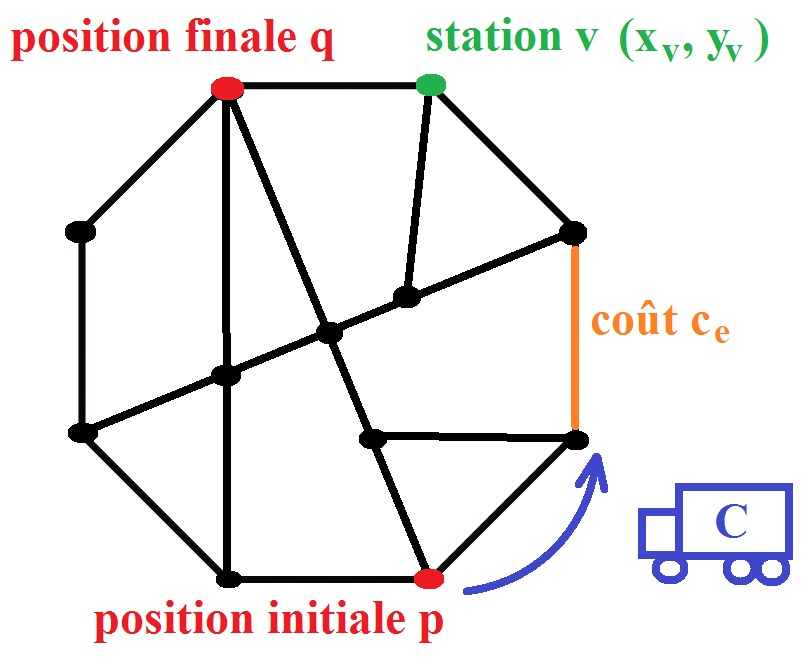
\includegraphics[width=\textwidth]{GrapheQuelconque.jpg}
      \end{center}
    \end{minipage}\hfill
    \begin{minipage}[c]{.5\linewidth}
      \textbf{Données.}
      \begin{itemize}
      \item graphe connexe $G=(V,E)$
      \item fonction de coût $\bs{c}$ sur les arêtes
      \item état initial $i$
        \begin{itemize}
        \item répartition initiale $\bs{x}$ des vélos
        \item position initiale du camion $p$
        \end{itemize}
      \item état cible $t$
        \begin{itemize}
        \item répartition cible $\bs{y}$ des vélos
        \item position finale du camion $q$
        \end{itemize}
      \item camion de capacité $C$
      \end{itemize}
    \end{minipage}
    
  \end{center}

  \pause
  
  \vfill
  \textbf{Tâche.} Trouver le coût minimal $\Upsilon_G$ de la séquence de mouvements permettant d'aller de l'état $i$ à l'état $t$ et le premier mouvement de cette séquence.

\end{frame}

\subsection{Résultats précédents}

\begin{frame}[label=PreviousResults]
  \frametitle{Résultats précédents}
  
  \begin{itemize}
  \item Graphe quelconque $\longrightarrow$ NP-difficile
  \item Graphe complet avec des coût unitaire $\longrightarrow$ NP-difficile
  \item \textcolor{red}{Arbre $\longrightarrow$ Linéaire en le nombre de sommets}
  \item Une borne inférieure du coût d'une solution optimale
  \end{itemize}

\end{frame}

\subsection{Cas étudié : le graphe circulaire}

\begin{frame}[label=GrapheCirculaire]
  \frametitle{Cas étudié : le graphe circulaire}
  
  \begin{center}
  
    \begin{minipage}[c]{.5\linewidth}
      \begin{center}
        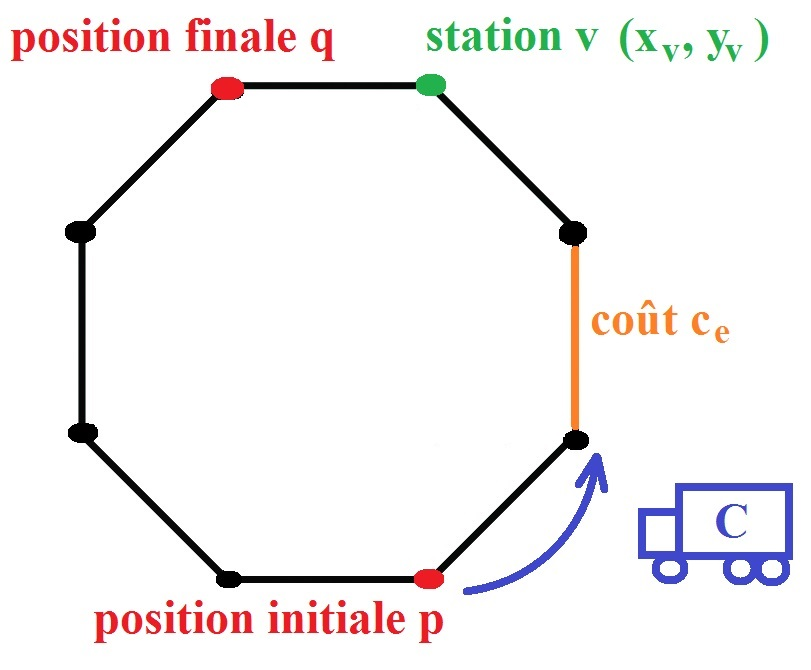
\includegraphics[width=\textwidth]{GrapheCirculaire.jpg}
        
        graphe \textcolor{red}{circulaire} $G=(V,E)$
      \end{center}
    \end{minipage}\hfill
    \begin{minipage}[c]{.5\linewidth}
      \textbf{Résultats obtenus :}
      \begin{itemize}
      \item Algorithme dans le cas triangulaire
      \item Algorithme polynomial dans le cas de la capacité infinie
      \item Conjecture dans un cas particulier de la capacité unitaire
      \end{itemize}
    \end{minipage}
    
  \end{center}

\end{frame}




\section{Algorithme polynomial pour une capacité infinie}

\subsection{Modèle et hypothèses}

\begin{frame}[label=CapaciteInfinie]
  \frametitle{Modèle et hypothèse}
  
  \begin{center}
  
    \begin{minipage}[c]{.5\linewidth}
      \begin{center}
        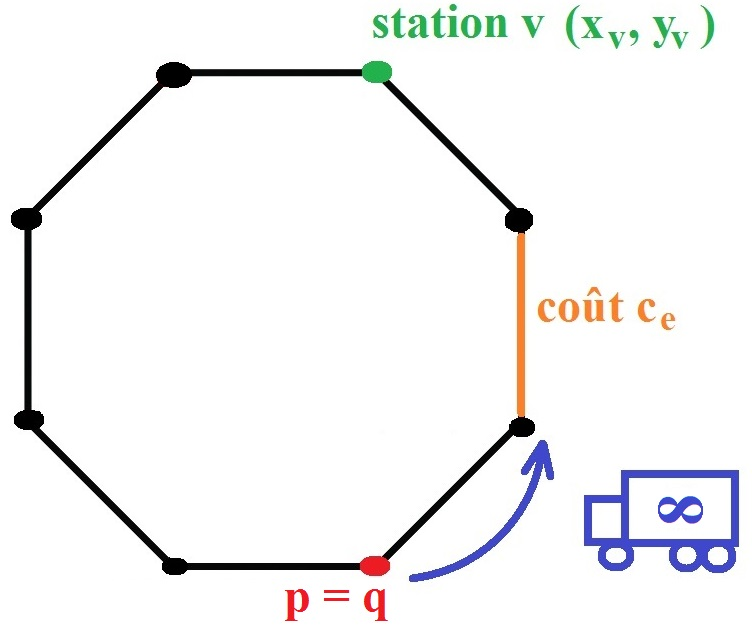
\includegraphics[width=\textwidth]{CapaciteInfinie/modele.jpg}
      \end{center}
    \end{minipage}\hfill
    \begin{minipage}[c]{.5\linewidth}
      \textbf{Hypothèses :}
      \begin{itemize}
      \item Capacité de transport $C$ infinie
      \item $p=q$
      \end{itemize}
    \end{minipage}
    
  \end{center}

\end{frame}

\subsection{Algorithme}

\begin{frame}[label=AlgoCapaciteInfinie]
  \frametitle{Idée générale de l'algorithme}
  \begin{center}
    \begin{minipage}[c]{\linewidth}
      \begin{minipage}[c]{.2\linewidth}
        \begin{overlayarea}{\textwidth}{0.28\textheight}
          \only<1>{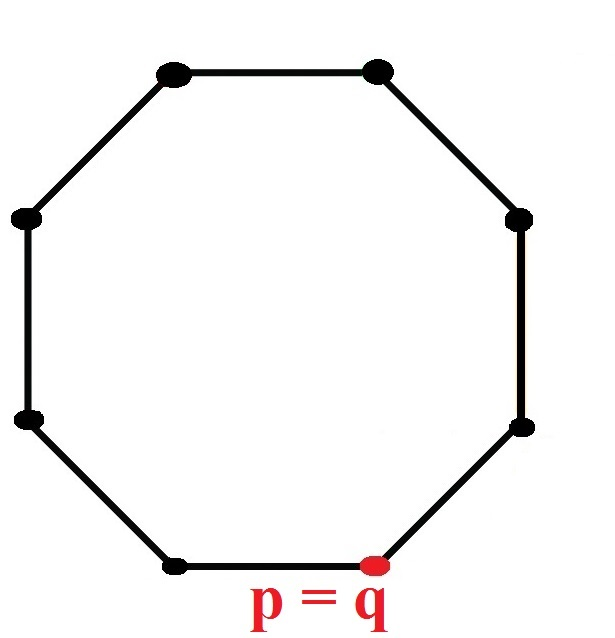
\includegraphics[width=\textwidth]{CapaciteInfinie/GrapheG.jpg}}
          \only<2>{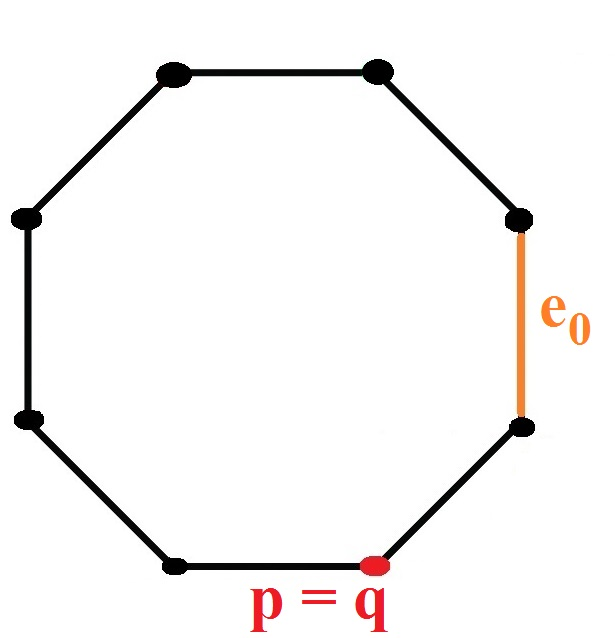
\includegraphics[width=\textwidth]{CapaciteInfinie/e0.jpg}}
          \only<3->{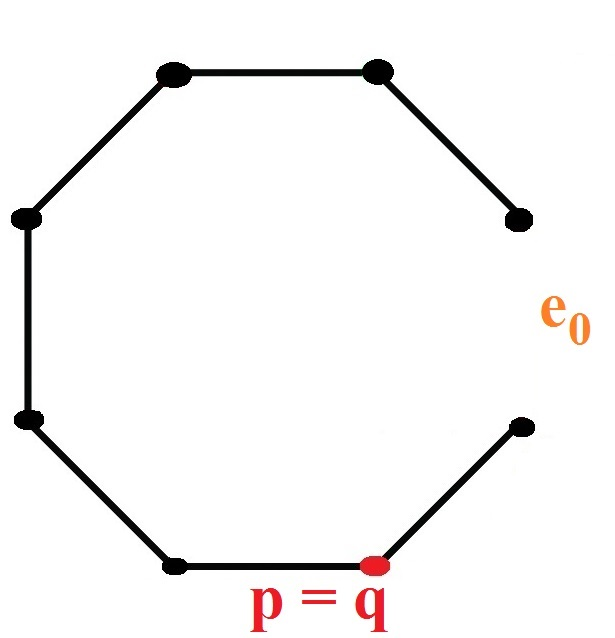
\includegraphics[width=\textwidth]{CapaciteInfinie/suppr_e0.jpg}}
        \end{overlayarea}
      \end{minipage}
      \begin{minipage}[c]{.8\linewidth}
        \begin{overlayarea}{\textwidth}{0.28\textheight}
          \begin{itemize}
          \item<2-> Pour chaque $e_0 \in E$
            \begin{enumerate}
            \item<3-> Construire $\bs{G(e_0)}$ en supprimant $e_0$
            \item<4-> Résoudre le SSBP sur $\bs{G(e_0)}$\\
            (algorithme dans le cas linéaire)
            \end{enumerate}
          \end{itemize}
        \end{overlayarea}
      \end{minipage}
    \end{minipage}
    \begin{minipage}[c]{\linewidth}
      \begin{minipage}[c]{.2\linewidth}
        \begin{overlayarea}{\textwidth}{\textheight}
          \only<5>{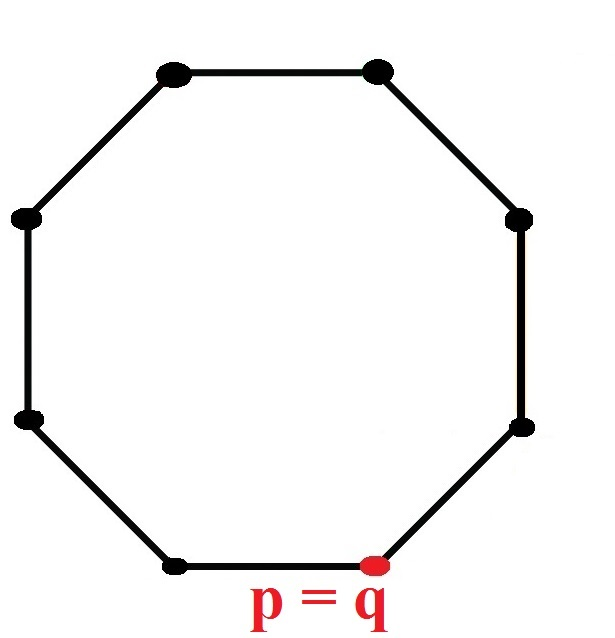
\includegraphics[width=\textwidth]{CapaciteInfinie/GrapheG.jpg}}
          \only<6>{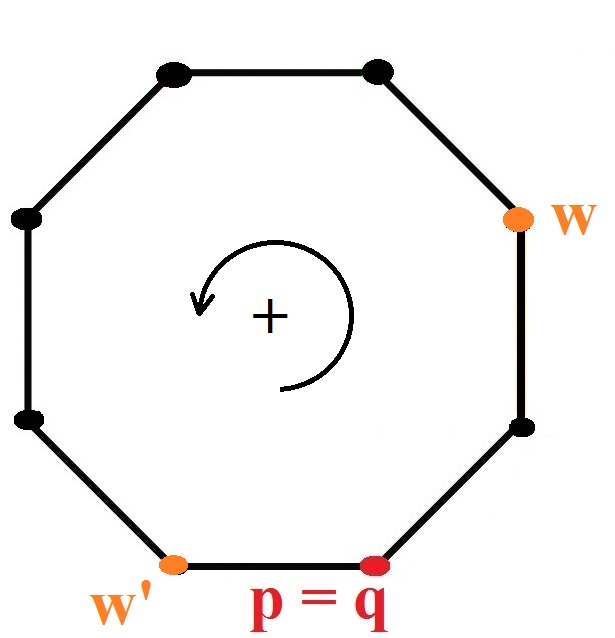
\includegraphics[width=\textwidth]{CapaciteInfinie/w.jpg}}
          \only<7>{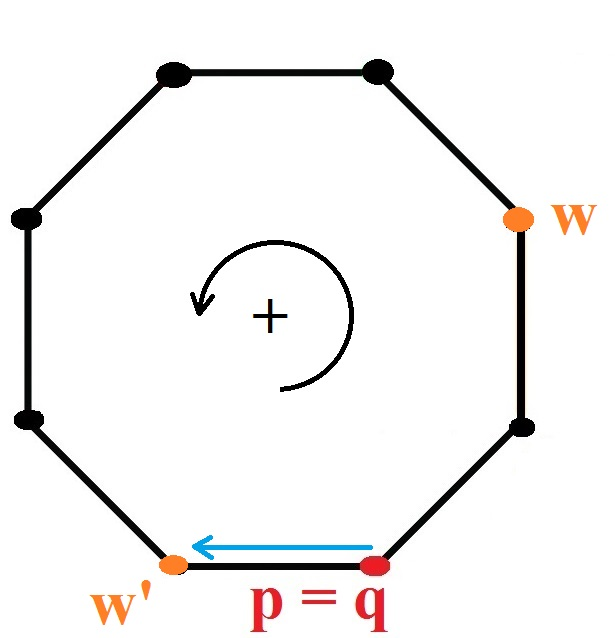
\includegraphics[width=\textwidth]{CapaciteInfinie/w_1.jpg}}
          \only<8>{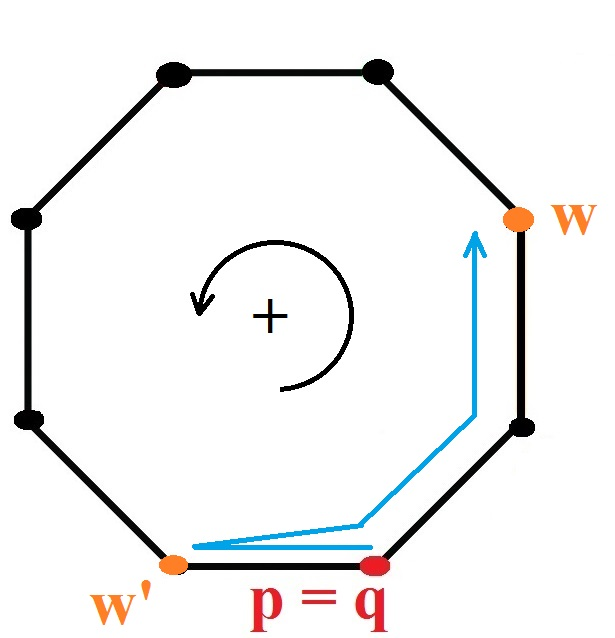
\includegraphics[width=\textwidth]{CapaciteInfinie/w_2.jpg}}
          \only<9>{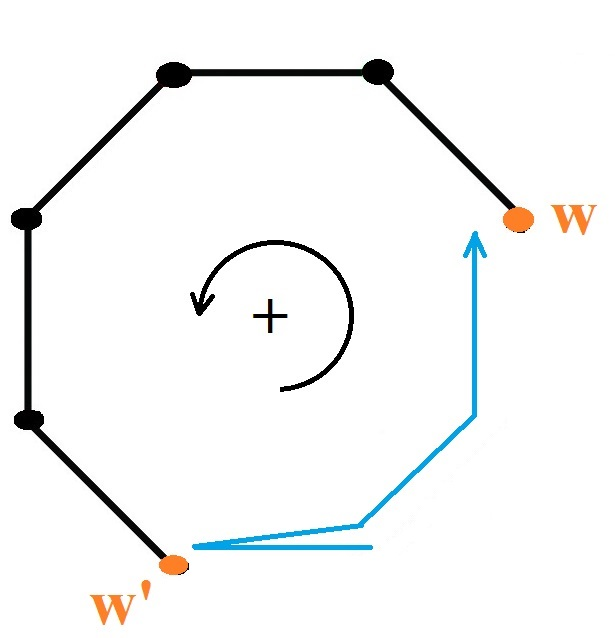
\includegraphics[width=\textwidth]{CapaciteInfinie/w_3.jpg}}
          \only<10>{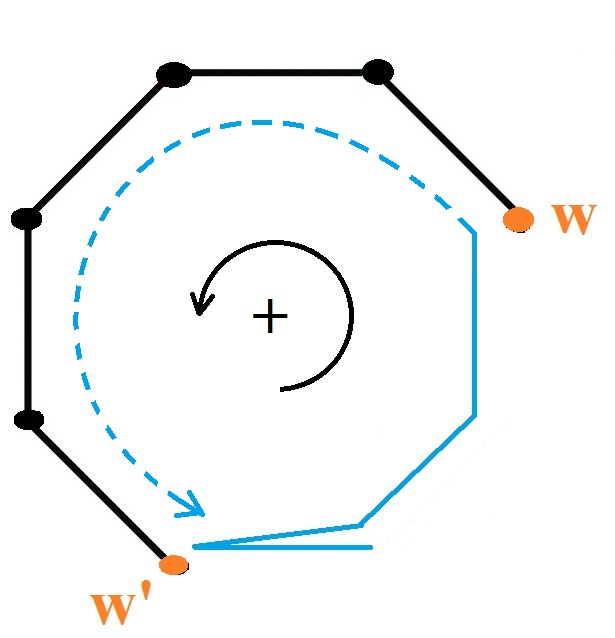
\includegraphics[width=\textwidth]{CapaciteInfinie/w_4.jpg}}
          \only<11>{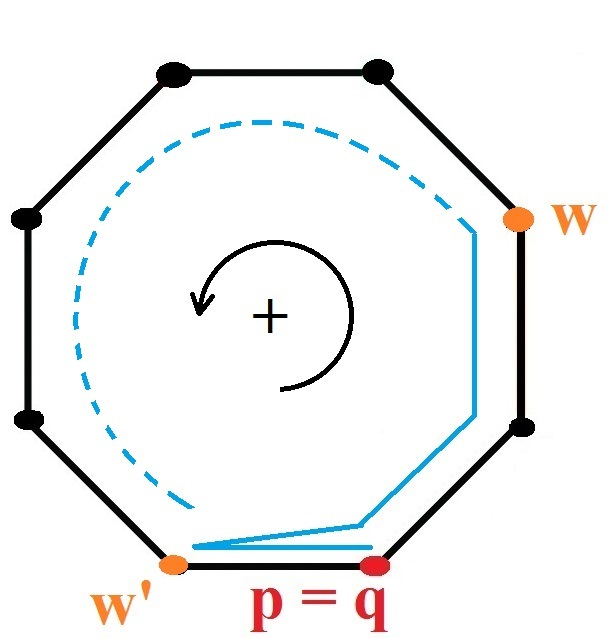
\includegraphics[width=\textwidth]{CapaciteInfinie/w_5.jpg}}
          \only<12>{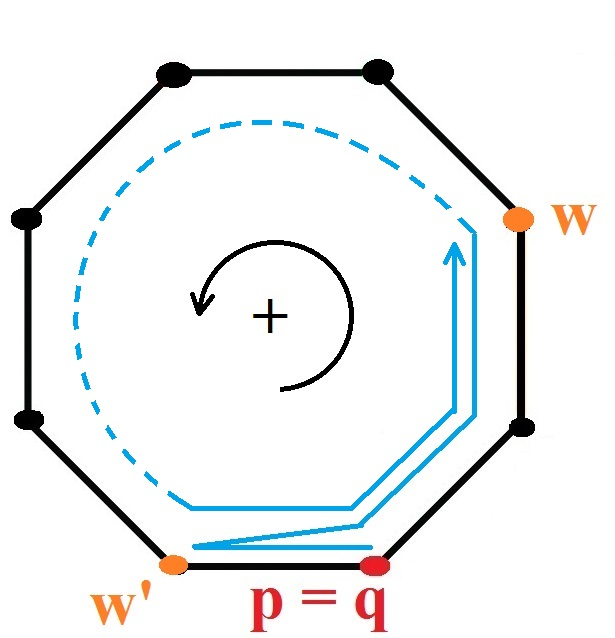
\includegraphics[width=\textwidth]{CapaciteInfinie/w_6.jpg}}
          \only<13->{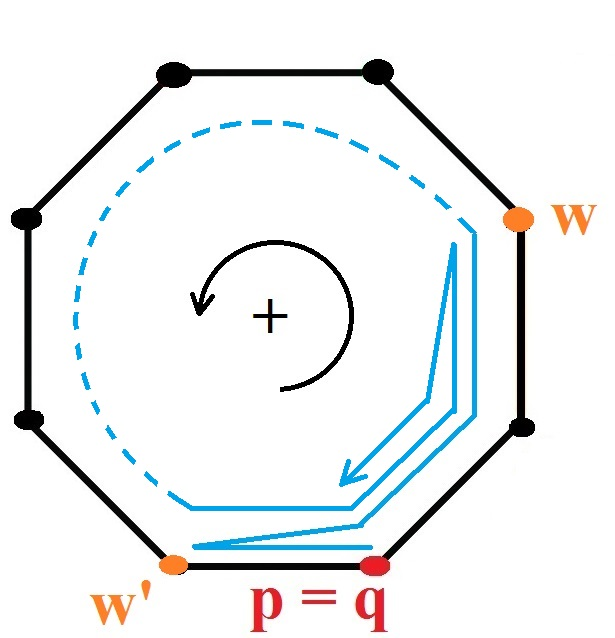
\includegraphics[width=\textwidth]{CapaciteInfinie/w_7.jpg}}
        \end{overlayarea}
      \end{minipage}
      \begin{minipage}[c]{.8\linewidth}
        \begin{overlayarea}{\textwidth}{\textheight}
          \begin{itemize}
          \item<6-> Pour chaque $w \in V$, pour chaque $w' \in ]w,o]_+$
            \begin{enumerate}
            \item<7-> aller jusqu'à $w'$ dans le sens $(-)$
            \item<8-> aller jusqu'à $w$ dans le sens $(+)$ en ramassant tous les vélos
            \item<9-> Construire le graphe linéaire $\bs{G(w,w',+)}$
            \item<10-> Résoudre le SSBP sur $\bs{G(w,w',+)}$\\
            (algorithme dans le cas linéaire)
            \item<12-> aller jusqu'à $w$ dans le sens $(+)$ en équilibrant toutes les stations
            \item<13-> revenir en $p$ dans le sens $(-)$
            \end{enumerate}
          \item<14-> Faire de même en allant d'abord sur $w$ dans le sens $(+)$
          \end{itemize}
        \end{overlayarea}
      \end{minipage}
    \end{minipage}
  \end{center}
\end{frame}

\begin{frame}[label=OptimaliteCapaciteInfinie]
  \frametitle{Complexité du cas de la capacité infinie}

  \begin{thm} \label{thm: optimalité algo infini}
  Il existe une algorithme cubique en le nombre de sommets résolvant le SSBP dans le cas où $C$ est infinie et où $p=q$.

  De plus, le coût $\Upsilon_{G}$ de la solution optimale est donnée par le minimum entre
  $$
    \min_{e \in E} \Upsilon_{G(e)}
  $$
  et
  $$
    \min_{w \in V, w' \in ]w,o]_+}
    \left(
      3 \sum_{ e \in E\left[ \left[w',w\right]_+ \right] }c_e + \min \left( \Upsilon_{G(w,w',+)} , \Upsilon_{G(w,w',-)} \right)
    \right)
  $$
  \end{thm}
\end{frame}

\begin{frame}
  \frametitle{Démonstration de la complexité du cas de la capacité infinie}
  \framesubtitle{Restriction du nombre de passages sur une arête particulière}

  \begin{overlayarea}{\linewidth}{\columnwidth}
  \only<1->{
  \begin{lem} \label{lem: passe au plus une fois par e0}
  Soit $S$ une solution optimale du SSBP dans le cas où $C$ est infinie et où $p=q$. Alors il existe une arrête $e_0 \in E$ tel que le camion passe au plus une fois par $e_0$.
  \end{lem}
  }
  \only<2->{
    \begin{proof}
      \begin{itemize}
        \item<3-> $\mbox{Coût}(S) < 2\sum_{e \in E}c_e$
        \item<4-> Par l'absurde, on ne peut passer deux fois par chaque arête.
      \end{itemize}
      \vskip-1\baselineskip
    \end{proof}
  }
  \end{overlayarea}
\end{frame}

\begin{frame}
  \frametitle{Démonstration de la complexité du cas de la capacité infinie}
  \framesubtitle{Restriction du nombre de passages sur l'ensemble des arêtes}
  
  \begin{lem} \label{lem: passe au plus 3 fois par chaque e}
  Soit $G=(V,E)$ un graphe circulaire. On suppose que la capacité $C$ du camion est infinie et que $p=q$.\\
  Alors il existe une solution réalisable optimale telle que :\\
  pour toute arête $e \in E$, le camion passe au plus trois fois sur $e$.
  \end{lem}

\end{frame}

\begin{frame}
  \frametitle{Démonstration de la complexité du cas de la capacité infinie}
  \framesubtitle{[Démonstration] Restriction du nombre de passages sur l'ensemble des arêtes}
  \onslide<1->
  {
    \begin{itemize}
    \item<1-> Deux cas :
      \begin{itemize}
      \item<2-> il existe $e_0 \in E$ tel que le camion ne passe pas par $e_0$
      \item<3-> le camion passe par tous les sommets et\\
      il existe $e_0 \in E$ tel que le camion passe exactement une fois par $e_0$
      \end{itemize}
    \end{itemize}
  }
  \onslide<4->
  {
    \begin{center}
      \onslide<4->
      {
        \begin{minipage}[c]{.4\linewidth}
        \begin{center}
          Solution initiale $S$\\
          \begin{overlayarea}{\textwidth}{\textheight}
            \only<4-5>{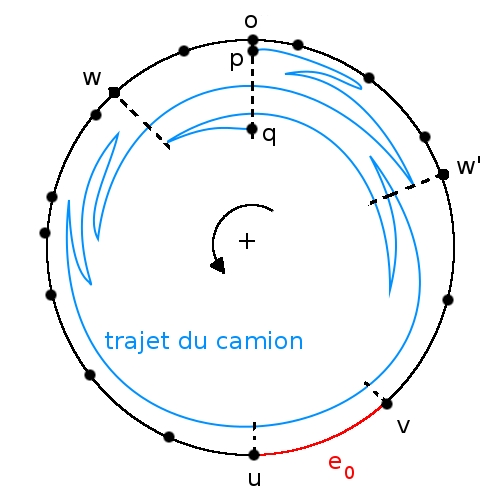
\includegraphics[width=\textwidth]{CapaciteInfinie/PreuveZeInf3.jpg}}
            \only<6>{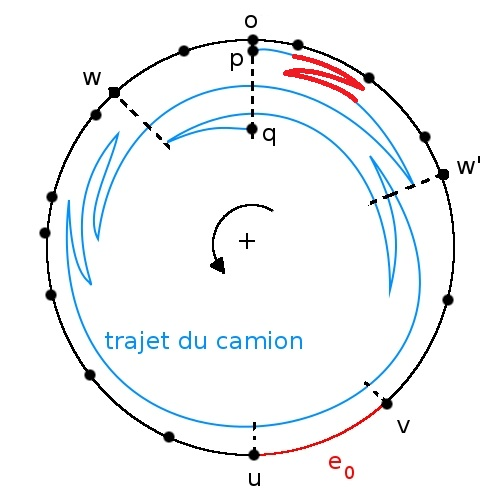
\includegraphics[width=\textwidth]{CapaciteInfinie/PreuveZeInf3_Zone1.jpg}}
            \only<7>{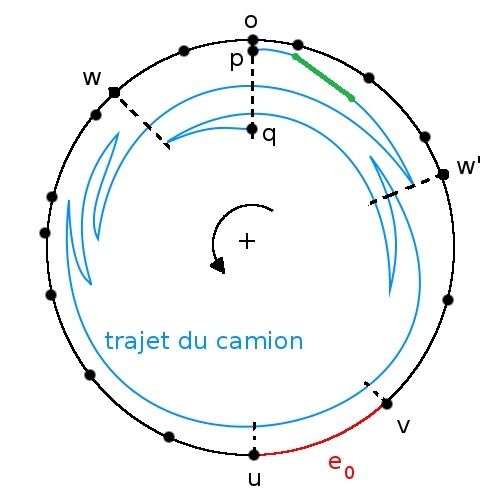
\includegraphics[width=\textwidth]{CapaciteInfinie/PreuveZeInf3_Zone1cor.jpg}}
            \only<8>{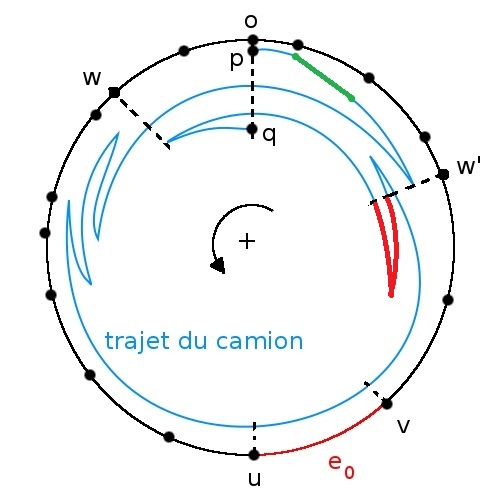
\includegraphics[width=\textwidth]{CapaciteInfinie/PreuveZeInf3_Zone2.jpg}}
            \only<9>{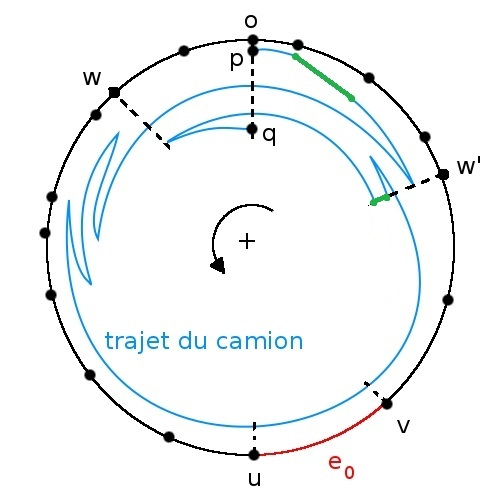
\includegraphics[width=\textwidth]{CapaciteInfinie/PreuveZeInf3_Zone2cor.jpg}}
            \only<10>{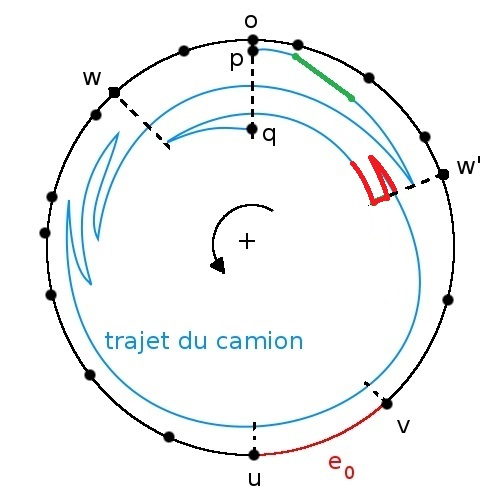
\includegraphics[width=\textwidth]{CapaciteInfinie/PreuveZeInf3_Zone3.jpg}}
            \only<11->{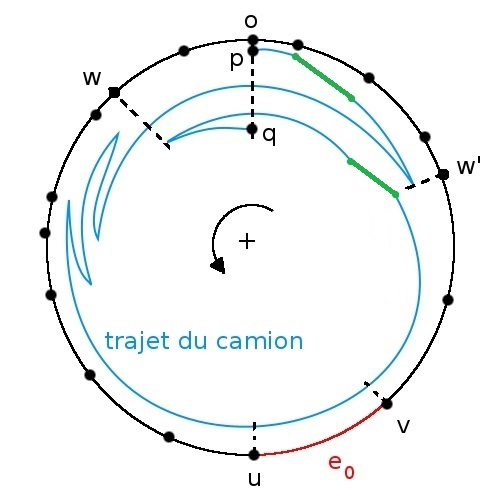
\includegraphics[width=\textwidth]{CapaciteInfinie/PreuveZeInf3_Zone3cor.jpg}}
          \end{overlayarea}
        \end{center}
        \end{minipage} \hfill
      }
      \onslide<5->
      {
        \begin{minipage}[c]{.4\linewidth}
        \begin{center}
          Nouvelle solution $S'$\\
          \begin{overlayarea}{\textwidth}{\textheight}
            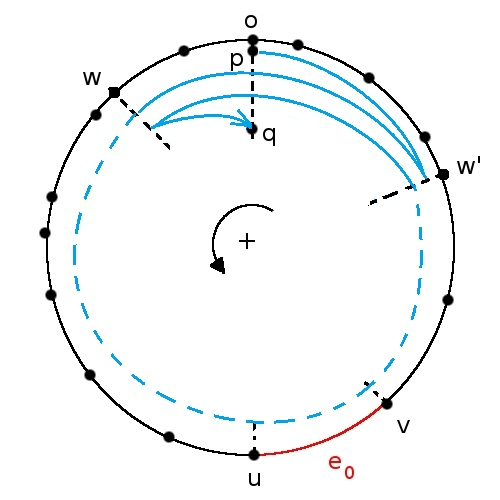
\includegraphics[width=\textwidth]{CapaciteInfinie/PreuveZeInf3_simple.jpg}
          \end{overlayarea}
        \end{center}
        \end{minipage} \hfill
      }
    \end{center}
  }
\end{frame}


\section{Conjecture dans un cas particulier de la capacité unitaire}

\subsection{Modèle et hypothèses}

\begin{frame}[label=CapaciteUnitaire]
  \frametitle{Modèle et hypothèse}
  
  \begin{center}
  
    \begin{minipage}[c]{.5\linewidth}
      \begin{center}
        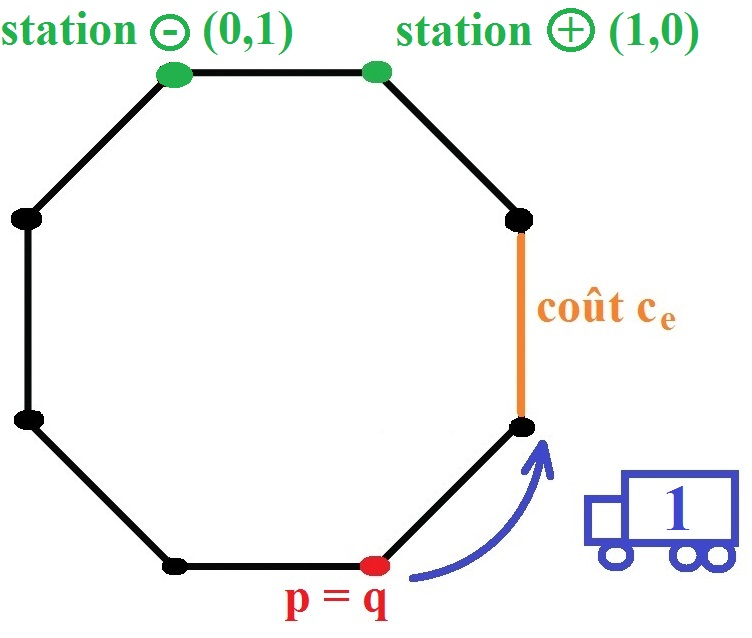
\includegraphics[width=\textwidth]{CapaciteUnitaire/modele.jpg}
      \end{center}
    \end{minipage}\hfill
    \begin{minipage}[c]{.5\linewidth}
      \textbf{Hypothèses (H) :}
      \begin{itemize}
      \item Capacité de transport $C=1$
      \item deux formes de stations possibles :
        \begin{itemize}
        \item station \plus de la forme $(1,0)$
        \item station \moins de la forme $(0,1)$
        \end{itemize}
      \end{itemize}
    \end{minipage}
  \end{center}
  \vfill
  \textbf{Conséquence :} $2n$ stations ($n$ \plus et $n$ \moins)
\end{frame}

\subsection{Conjecture et algorithme polynomial}

\begin{frame}
\frametitle{Conjecture et algorithme polynomial}

\onslide<1->
{
  \begin{conj} \label{conj: capacité unitaire - un passage}
  Sous les hypothèses (H), il existe un trajet optimal et une arête $e_0$ tels que le camion passe au plus une fois par $e_0$ au cours de ce trajet.
  \end{conj}
}
\onslide<2->
{
  \begin{thm} \label{thm: capacité unitaire - optimalité}
  Sous les hypothèses (H) et en supposant la conjecture précédente vraie, il existe un algorithme polynomial donnant le trajet optimal du camion.
  \end{thm}
}
\end{frame}

\begin{frame}
\frametitle{Idées clés de la démonstration}

\begin{proof}
  \begin{itemize}
  \item<1-> il existe $e_0 \in E$ tel que le camion ne passe pas par $e_0$
  \item<2-> le camion passe par tous les sommets et\\
    il existe $e_0 \in E$ tel que le camion passe exactement une fois par $e_0$
    \begin{itemize}
    \item<3-> Construire le graphe biparti complet (\plus et \moins)
    \item<4-> Recherche de cycle hamiltonien optimal $\Rightarrow$ indépendant origine
    \item<5-> On résout à partir de la station atteinte après le passage sur $e_0$\\
    (algorithme dans le cas linéaire)
    \end{itemize}
  \end{itemize}
  \vskip-1\baselineskip
\end{proof}
\onslide<5->
{
  \begin{center}
    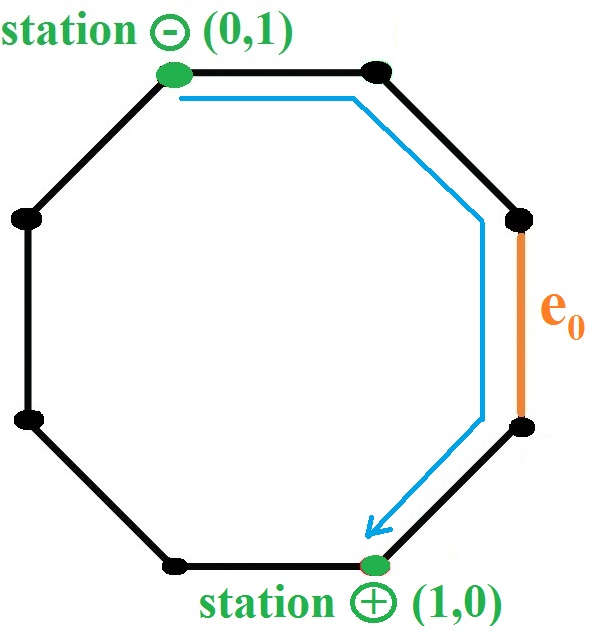
\includegraphics[width=0.35\textheight]{CapaciteUnitaire/PreuveAlgo1.jpg}
    \hspace{2cm}
    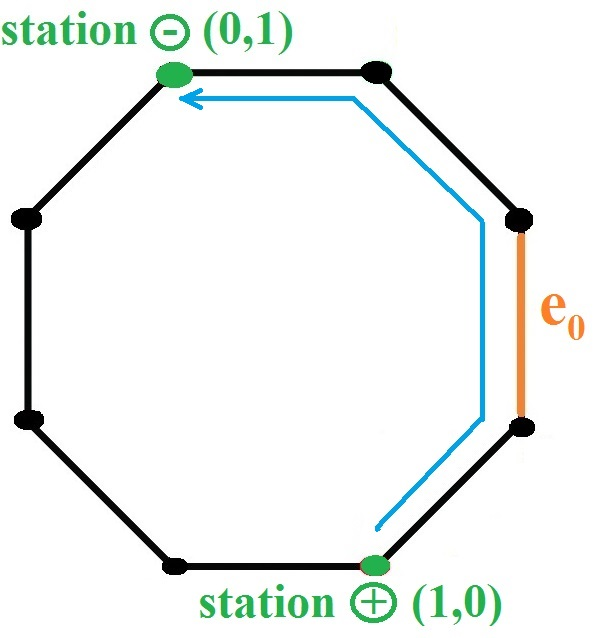
\includegraphics[width=0.35\textheight]{CapaciteUnitaire/PreuveAlgo2.jpg}
  \end{center}
}

\end{frame}


\subsection{Majoration du coût et polynomialité}

\begin{frame}
\frametitle{Majoration du coût et polynomialité}
\onslide<1->
{
  \begin{prop}
  Sous les hypothèses (H), si  $\Upsilon_G$ < $2\sum_{e \in E}c_e$, alors il existe un algorithme polynomial donnant le trajet optimal du camion.
  \end{prop}
}
\onslide<2->
{
  \begin{proof}
  Par l'absurde, si $S$ passe au moins deux fois par chaque arête
  
  alors $\Upsilon_G~\ge~2\sum_{e \in E}c_e$
    \vskip-0.8\baselineskip
  \end{proof}
}

\end{frame}


\end{document}
